%Import the Thesis formatting
\documentclass[11pt]{ucthesis}

%Package Imports
\usepackage[pdftex]{graphicx}
\usepackage{parskip}
\usepackage{url}
\usepackage{titlesec}
\usepackage{hyperref}
\hypersetup{
	colorlinks,
	citecolor=black,
	filecolor=black,
	linkcolor=black,
	urlcolor=black
}

\titleformat{\part}
	{\normalfont\fontsize{12}{12}\rm\center}{}{1em}{}
\titleformat{\chapter}
{\normalfont\fontsize{12}{12}\rm\center}{\thechapter}{1em}{}
\titleformat{\section}
	{\normalfont\fontsize{12}{12}\rm}{\thesection}{1em}{}
\titleformat{\subsection}
	{\normalfont\fontsize{12}{12}\rm}{\thesubsection}{1em}{}

\begin{document}
\title{Analysis of Various Algorithmic approaches to Software-Based 1200 Baud Audio Frequency Shift Keying Demodulation for APRS}
\author{Robert F. Campbell}
\degreemonth{June} \degreeyear{2016} \degree{Master of Science}
\defensemonth{May} \defenseyear{2016}
\numberofmembers{3} \chair{John Bellardo, Ph.D.\newline
Associate Professor, Computer Science}
\othermemberA{Bridget Benson, Ph.D.\newline
Assistant Professor, Electrical Engineering}
\othermemberB{Dennis Derickson, Ph.D.\newline
Department Chair, Electrical Engineering}
\field{Computer Science} \campus{San Luis Obispo}
%\copyrightyears{seven}
\maketitle

\begin{frontmatter}

\copyrightpage

\committeemembershippage

\begin{abstract}
Digital communications continues to be a relevant field of study as new technologies appear and old methodologies get revisited or renovated. The goal of this research is to look into the old digital communication scheme of Bell 202\,\cite{stauffer1984fsk} used by APRS and improve software based demodulation performance. Improved performance is defined by being able to correctly decode more packets in an efficient, real time, manner. Most APRS demodulation is currently done using specialized hardware since that yields the best performance. This research shows that through using Sivan Toledo's javAX25\,\cite{javax25github} software package, new demodulation algorithms can be implemented that decode more Bell 202 encoded AX.25 packets than the existing software could. These improvements may help drive the adoption of software demodulation since it is a low cost alternative to specialized hardware.
\end{abstract}

\tableofcontents
\listoftables
\listoffigures

\end{frontmatter}

\addtocontents{lof}{Figure ~\hfill Page \par}
\addtocontents{lot}{Table ~\hfill Page \par}
\addtocontents{toc}{\vskip 0.4em CHAPTER\par}

\chapter{Introduction}

Amateur Radio Operators, commonly referred to as "hams," make the best of what resources they have available to them. However, once something is working a "don't touch it if it ain't broke" approach is often taken. Between these two mentalities some interesting phenomenon have occurred within the ham community. For example, some radio systems that are in active use today have only seen very minimal attention since the 1980's when they were originally installed. On the flip side of leaving things alone, hams are very quick to take advantage of a good deal or opportunity when they are presented one.The implementation and development of the Automated Packet Reporting System (APRS) is no exception to the way hams approach things \cite{Bruninga}. Much of this system is based off older hardware and protocols - from the 1980s - that was readily available and few improvements have been made, and although the specification has been relatively stable there are inconsistencies. These inconsistencies include varying implementations from vendor to vendor as well as portions of the specification that are not clearly defined resulting in vastly inconsistent performance \cite{KWFThesis, KWFTAPR}.

%A recent scenario that expresses both of these characteristics of hams is when the Federal Communications Commission (FCC) required that public service agencies such as police, fire, and ambulance go to narrow banding (a 12.5kHz channel from a 25kHz channel). This change was needed to be able to support more channels in the limited radio frequency spectrum \cite{Commission2012}. Due to this change a lot of equipment became available that could not do narrow banding, which many hams sprung at the opportunity for. In addition to showing their need to take advantage of a good opportunity, it also shows that they do not feel the need to upgrade their systems even though there are congested areas that would benefit immensely from narrow banding.

So, what is APRS, and why does it matter? A brief introduction to APRS is that it is a digital communication scheme used by hams where a packet (whose content is varied, but is usually a GPS position - which is what gave APRS it's original name "Automated Position Reporting System"\cite{WikiAPRS}) is sent out over radio. A major challenge to this protocol and method of digital communication is the fact that it uses radio, which is susceptible to interference, weak signals as the distance from the transmitting station increases, as well as a myriad of other items. This research focuses specifically on the receiving end of these signals in order to see what improvements can be made to software based approaches to decoding - demodulating - these packets.

The reasoning for trying to make improvements in software based demodulation are many, but a few of the more motivational ones are to follow. One advantage of doing software based demodulation is that it removes the necessity of specialty hardware; Instead of having dedicated hardware whose sole purpose is to modulate and demodulate APRS packets, hams can use a computer to do these tasks. By using a computer's sound card, audio from the radio can be processed using software to decode received packets, or audio can be played from the sound card to the radio to be transmitted. With the abundance of personal computers, this can provide a much cheaper solution for hams who are interested in trying out APRS without having to put down a potentially big initial investment (\textasciitilde\$200 \cite{Kantronics2014,Outlet2014}) for a piece of hardware that serves one purpose. The price of this specialty hardware is steep and it is limited to only performing communication on a single channel. When using a line in / out on a computer they are typically stereo meaning that a single sound card could handle operations on multiple channels. If two channels just is not enough the capabilities of a computer demodulator can be expanded my merely adding another sound card which is relatively cheap at \textasciitilde\$20 \cite{Newegg}. To perform communication on 4 channels using dedicated hardware the cost would be $800! For this cost a whole computer with a half dozen sound cards could be purchased, only further expanding capabilities.

%Another cost advantage is when multiple APRS networks are operated alongside each other. For some events that hams assist with, GPS tracking is used to keep track of assets, such as support vehicles, ambulances, water trucks, etc. In order to get more frequent position updates the traffic can be moved from the primary transmit frequency to a different back haul frequency to alleviate some of the Radio Frequency (RF) congestion. If there are multiple back haul frequencies - three, for example - in addition to the primary transmitting frequency, there would be a total of four frequencies carrying APRS traffic that need to be monitored and the traffic demodulated. Instead of spending \$800 to get four dedicated units for APRS to handle all of the traffic an extra sound card could be purchased for a computer (\textasciitilde\$20 \cite{Newegg}). Since audio inputs are typically stereo with a left and a right channel, these can be considered as two separate audio inputs since the radio transmissions are mono (single channel). Hence, between the input that the computer already has and the new one added through the extra sound card, there could be a total of four audio input channels on the computer which the audio from the radios can be piped into.

In addition the the price advantages of software based demodulation approaches there is also one other primary advantage. If software is being used instead of hardware there is the potential for a lot more capabilities since processing power and available memory increase drastically. For instance, on one of the dedicated hardware solutions, the Kantronics KPC-3 Plus, has a mere 512KB of memory compared to that of any computer which is over 4GB as of 2014 - and that is just the ram, not the hard drive space \cite{Kantronics2014,Graham-Smith2014}. Additionally, instead of just being able to handle live events and process each data point in the best manner possible as soon as it comes in, post processing becomes an option.

With the cost and versatility of a software demodulation solution now introduced, the paper addresses the following: Chapter 2 goes into background information, with a deeper introduction to APRS and a presentation of the aspects important to understanding this research. In Chapter 3, some of the current methods for interfacing with APRS, both hardware and software, are explained. Demodulation techniques are discussed in Chapter 4. Chapter 5 talks about the challenges of demodulating APRS packets. Chapter 6 discusses the methods used for benchmarking and comparing the demodulators. In Chapter 7, information on how the demodulators and algorithms are tested is presented. Chapter 8 goes into more detail about the implementations in this project. Chapter 9 discusses the results of both the newly implemented algorithms and compares them to other demodulators. Areas of additional research and future work are discussed in Chapter 10. Chapter 11 is concluding remarks.

\chapter{APRS Background and Definitions}
From the introduction it is known that APRS is a method of digital communication used by hams in order to inform other hams of their location. In addition to supporting sending positions, APRS can be used to send messages, bulletins, weather, and other information. Since these packets are transmitted via radio  - which has limited coverage - APRS can be viewed as a local area awareness network. This gives hams who are listening for and decoding APRS packets information about nearby transmitting stations. This brief overview should give a little insight into APRS, but the rest of the section will focus more on what is going on behind-the-scenes to explain how APRS works in terms of the protocols, data transmission, modulation, etc.

In order to organize this discussion of the different components of APRS let us break it down into the Open Systems Interconnection (OSI) model representation. However, before fitting it into the OSI model here is a brief reminder of the relevant layers that are going to be discussed. Layer 1 of the OSI model is the physical layer. The physical layer consists of everything that is used to transport one bit of information from one location to another. The second layer is the data link layer. Within the data link layer bits from the physical layer are passed up to the network layer, and information from the network layers is framed and handed off to the physical layer. Layer 3 is the Networking layers. This Layer is responsible for determining the path that packets will take and providing flow control to prevent flooding. Above these layers are layers 4-7 which are the transport, session, presentation, and application layers respectively \cite{Sosinsky2009}. These upper layers get too inter-tangled to be able to cleanly separate them. For instance within the AX.25 2.2 specification a TNC is mentioned that only implements layers 1, 2, and 7 of the OSI model \cite{Beech1998}.

Here is the best division of APRS into the OSI model, following introducing this division each layer will be individually discussed in more detail. Layer 3 of the OSI model for APRS is the the AX.25 Protocol,  High-Level Data Link Control (HDLC) protocol composes layer 2. All the way at the bottom, layer 1 for APRS consists of the Terminal Node Controller (TNC) and Radio \cite{Silver2013}. A brief note on why the discussion begins with Layer 3 is because this is how the data is transferred. The interest stop here and does not continue to the layers above layer three, because those are all application specific. Starting with AX.25 the background information will be given down to Layer 1 which is where this research actually aims to make a contribution.

\section{Layer 3 - AX.25}
Layer 3, the network layer, is responsible for routing frames between individual nodes in the network. A frame of data is more traditionally called a packet at this point since AX.25 is a packet switched network protocol \cite{Peterson2011}. AX.25 is the amateur X.25 protocol. Meaning that the AX.25 protocol, which is what APRS uses, was developed my Amateur radio operators and is based off of the x.25 protocol. Since the origins of AX.25 lie within X.25, the discussion will begin with X.25. 

\subsection{X.25}
Developed in the 1970s the packet switching protocol X.25 was deployed on telephone networks where it was used until it began to be displaced by the IP protocol. The X.25 protocol suite provides OSI layers 1-3, although it does have standards that support each of those layers \cite{Sosinsky2009}. For instance the X.21 standard is commonly used for layer 1 of X.25 and ISO 7776 specifies a Link Access Procedure Balanced (LAPB) to assists with layer 2, the data link layer \cite{Gallagher1997}. The Data Link layer of LAPB, a bit oriented protocol derived of HDLC,  manages packet framing and ensures that frames are error free and properly sequenced. When used on telephone networks there were five distinct modes that the protocol would operate in: Call setup for establishing the connection, Data transfer, idle where the connection is established but no data is being transferred, call clearing for terminating the connection, and restart for resynchronizing the host and client \cite{Javvin2006}. Many of the features of the Layer 2 and Layer 3 operations of X.25 can be found in at least a similar fashion in AX.25.

\subsection{AX.25}
Next the AX.25 protocol will be discussed through comparison and contrast with X.25. One of the main differences between the X.25 and AX.25 is that when the specification is read, in addition to specifying the behavior of Layer 3, the behavior of Layer 2 is also included. Although this is somewhat implied for X.25, there are still separate documents for the specifications for each one of the layers. After reading the specification for AX.25 it very clearly defines the framing with starting and terminating flags as well as the networking and routing \cite{Beech1998}.

\section{Layer 2 - High-Level Data Link Control}
Layer 2 of the OSI model which is responsible for framing the bits, or packets, from layer 3 is taken on my HDLC in APRS. The goal of HDLC is to make sure that when the data is received and passed up to Layer 3, that it is error free, without loss, and in the correct order \cite{Javvin2006}. There are a few ways that HDLC accomplishes this, two of which are framing and with the Frame Check Sequence (FCS). The framing occurs through the use of flags around the data. A flag is one byte and is hex 0x7E. For APRS common practice is to send multiple flags consecutively to give transmitting radio time to key up and settle or to give receiving radios time for their squelch to open. Since it is an non-return to zero inverted (NRZI) encoding no change in frequency corresponds to a 1 and a change in frequency corresponds to a 0. As such multiple 1s in a row make it hard to keep timing which is why bit stuffing is used. With the exception of the flag which contains six consecutive 1s (0x7E = 01111110) if there six or more consecutive 1s in the data packet a zero will be stuffed after the fifth 1 to increase the clocking energy in the signal.

\section{Layer 1 - The Bell 202 Modulation and the Radio}
Since Layer one is composed of the things needed in order to transmit one bit from one location to another, it needs to be made clear what all this includes for APRS. Starting with air, the medium through which the radio frequency (RF) signals propagate, the RF transmissions are received or transmitted by the radio. Without decomposing the radio into all of its individual components, the audio that the radio receives then has to be processed. In order to stay focused on what happens in layer 1 and not start mixing the other layers together some more discussion of what this audio signal consists of is necessary.

The audio signal that contains the APRS packets is composed using the Bell 202 modulation which is an Audio Frequency Shift Keying (AFSK) mode. As such RF either comes in through the radio, is translated to the corresponding audio, and then demodulated into a bit stream by interpreting the Bell 202 modulation. Or, a bit stream from layer 2 of APRS is modulated using the Bell 202 modulation, this modulated audio is passed to the radio, and the radio then transmits it out. Since decomposing the radio down into its individual components does not have any affect on representing the different OSI layers of APRS, it will not be discussed. However there are factors that affect wireless communications and RF signals that will be discussed in chapter 4.

\subsection{Frequency Shift Keying}
In order to understand the Bell 202 modulation scheme the communication mode of AFSK needs to be introduced. AFSK is a form of frequency shift keying (FSK) that occurs by modulating frequencies in the audible range. FSK uses multiple frequencies in order to represent the different symbols such as 1 or 0 or mark and space in our case. If the frequency of the data carrying signal can be determined, then the symbol is knows for that bit period. FSK is the more generic term and is used for 9600 baud (bits per second) APRS on Ultra High Frequencies (UHF). In this mode the actual RF carrier in the 440MHz band is modulated between one frequency and another nearby frequency in order to represent the two different symbols. In contrast, AFSK switches between two different audio signals, which for APRS on Very High Frequencies (VHF) is then modulated onto the RF carrier using Frequency Modulation (FM).


\subsection{Bell 202}
With FSK and AFSK now introduced the AFSK used within Bell 202 can be described. The Bell 202 modem was patented in 1984 using 1200Hz and 2200Hz tones, although the patent was originally filed in 1981 \cite{stauffer1984fsk}. Interestingly, the International Telecommunication Union (ITU) did not publish a standard for this modulation that were used in telephone networks until 1988. In the standard, however they use 1300Hz tone for symbol 1 and 2100Hz tone for symbol 2 called a mark and space respectively \cite{ITUV23}. The original bit stream is modulated using a non-return to zero inverted (NRZI) encoding. This means that when a transition occurs from one symbol to another in the Bell 202 modulated signal this symbolizes a 0 bit in the original data bit stream and if the Bell 202 symbol remains constant over multiple symbol periods, that signifies a 1 bit in the original data bit stream. For Bell 202 the frequencies that are used are 1200Hz and 2200Hz tones for the mark and the space as opposed to the 1300Hz and 2100Hz tones proposed in the ITU specification.
\begin{Figure}
  \centering
	\includegraphics[width=0.75\linewidth]{Datasignalencodingbitstream0000.png} 
	\captionof{figure}{Example Bell 202 signal encoding the bit stream '0000'.}
\end{Figure}
\chapter{Approaches to Utilizing the APRS Network}
In the world of APRS there are many solutions that hams take advantage in order to utilize the network. Some they find and make work, some they purchase to use exclusive for APRS, and some go through the trouble of inventing their own solutions. This chapter explains some of the common systems used on the APRS network, primarily those that can be used for receiving, starting with terminal node controllers and progressing to software based demodulation.

\section{Terminal Node Controllers}
Currently there are many systems that will demodulate these Bell 202 encoded APRS packets. The original hardware used for this communication style was dedicated modems similar to dial-up 56k modems that did the encoding and decoding. These modems were connected directly to the radio and the radio would let the modem know through a signal pin if the radio was receiving what it thought was a data carrying signal. And conversely, the terminal node controller (TNC), a modem used in AX.25 operation, would let the radio know by signalling the radio to transmit when it had data to send out \cite{Wolfgang2005}. Just as a reminder of the age of the technologies that are being used for the data transport of APRS, packet radio originated around 1985 as TNCs became affordable \cite{Helms1992}. This means that this technology is 30 years old at the time of writing in the year 2015.

With a radio and a TNC, amateur packet stations and digipeaters (digital packet repeaters) are possible \cite{Group2012,Wiki2012}. Digipeaters are an essential part of the ham packet network, but many users wish to report their GPS position onto the APRS network instead of just relaying traffic for other stations. In order to accomplish this, a GPS receiver is required. Now, stations can take the data from their GPS receiver and put it in the payload of the APRS packet and transmit the GPS reported position onto the network. One other common use of a TNC is an internet attached digipeater, usually though the use of a computer, that would allow the data to be posted to the APRS-IS servers \cite{Community2015}. Just to give an example of some of the TNCs available, those within the testing testing scope of this project will be listed. There are eight - six unique models - whose decoding results are compared to the software approaches. These modems included the two AEA PK-88s, two Kantronics KAM Pluses, a Kantronics KAM, an MFJ-1278, a PK-232, and a PK-232MBX. An example image of what a TNC looks like, the photo features a KAM Plus can be seen in Figure \ref{kantronicsKamPlus}. Although these modems work for decoding and encoding Bell 202 packets, this is not their only purpose as they are multiple mode modems and support numerous other transmission modes and modulation schemes, so just a note that these are modems that happen to be used for and work with APRS.

\begin{figure}
  \centering
	\includegraphics[width=0.75\linewidth]{images/Kantronics-KAM-Plus.jpg} 
	\caption{Image of the Kantronics Kam Plus \cite{KK6RF}}
   \label{kantronicsKamPlus}
\end{figure}

\section{Specialized APRS Hardware}
Many people know exactly what they would like to do with APRS and exactly what traffic they want to contribute to the APRS network. This has allowed for companies to start commercially making dedicated APRS hardware, since there is a demand for it. In addition to making this hardware available the producers support the hardware and make pretty user interfaces for the users to be able to program the hardware exactly as they like and without having to invest much time into understanding how different components work together. Some examples of APRS exclusive devices are ArgentData�s OpenTrackers (Figure \ref{openTracker3}), Byonics� TinyTrack, and Fox Delta�s Fox Track \cite{Miller,Byonics,Foxtrak}. These compact packages along with a radio and a GPS module perform APRS tasks at a satisfactory level for many users.

\begin{figure}
  \centering
	\includegraphics[width=0.75\linewidth]{images/Ot3m-termblk.jpg} 
	\caption{Image of Argent Data's Open Tracker 3. \cite{Data}}
   \label{openTracker3}
\end{figure}

Since the average user only wants to report positional information, these dedicated devices are simple to setup to do such but also only include a simple feature set. Although these trackers contain some features, since they are all small embedded systems they can not and do not have implemented all of the features that APRS supports. An example is the messaging service. Since these devices don�t have a display or a keypad, there is no way to input or display a message. Certain radio manufacturers have begun to integrating the TNCs into the radios themselves to utilize the radio�s screen. The Kenwood TM-D700 series and Yaesu FTM-350 (Figure \ref{yaesuFTM350}) are examples \cite{Kenwood,Yaesu}.

\begin{figure}
  \centering
	\includegraphics[width=0.75\linewidth]{images/FTM-350US_F.jpg} 
	\caption{Image of the FTM-350 Radio which has APRS integrated. \cite{Yaesua}}
   \label{yaesuFTM350}
\end{figure}

However, both the options in this section and the one previous on TNCs require going out and buying special hardware in order to perform APRS whether it be a TNC itself of a OpenTracker. This can be expensive and cost prohibitive for some hams to be able to begin APRS operations.

\section{Software Based Demodulation}
It can be assumed that before a ham operator becomes interested in the APRS network and sending APRS packets that they will already have a radio. So, if they already have a radio all they have to do is buy a piece of hardware that will do the modulation in order to send a packet. However, hardware costs money and before diving right in it might be nice to get their feet wet first. A good, cheap alternative to dedicated hardware is to use hardware that hams already have. A good choice that will fit the needs is a computer, which most hams probably own at least one of. On this computer amateurs can build or buy a cheap interface to a radio, around \textasciitilde\$15 instead of \textasciitilde\$150 for a piece of dedicated hardware, and then use software to do the modulation and demodulation.

This seems to be a route that some are taking and a demodulation scheme that this project explores in detail, but first some more information on current systems that operate in this software realm. Some examples of the software that can be used are George Rossopoylos�s Packet Engine \cite{Rossopoylos}, Thomas Sailer�s Linux Sound Modem \cite{Sailer1997,Sailer2000}, or Sivan Toledo's javaAX25 \cite{javax25github, Toledo2012a}. On a computer, even ones with minimal resources, there are algorithms that are being used to demodulate the APRS packets. Again, what this project aims to investigate is what improvements can be made to the algorithms and software based demodulation approaches in order to decode these packets in a more robust fashion and to try and get similar performance to TNCs and dedicated hardware. This is based on observations in initial analyses where software was unable to decode packets, the hypothesis was made that improvements can be made to software based demodulation. It is worth mentioning here that the Toledo's javaAX25 will be the software basis that will be developed on top of, so more information is to follow.

\subsection{javaAX25}
Sivan Toledo's javaAX25 is one method of utilizing the APRS network. Toledo's software is very comprehensive in handling the encoding, decoding, radio control, and interfacing with sound cards to allow for full use of APRS using this software. However in addition to just being able to utilize APRS there is also a test application inside of this package that allows for quick and easy testing of everything in the suite - of the most interest, however is the ability to be able to test demodulators. Although all of these features were included, the three primarily used in this project were the modulation, demodulation, and demodulator testing. Due to its extent and its ease of access on line through Github, this was chosen to be the basis for this project \cite{javax25github}. For a complete list of features the manual can be found in the following reference, and even from the beginning the mission statement that he outlines coincides with that of this research \cite{Toledo2012a}.

Toledo did some benchmarking of his software and found that running two demodulators in parallel provided the best results. The demodulators were exactly the same, the only difference is that one was processing data after a bandpass filter that was just centered around the two frequencies of interest, and the other had a bandpass filter that in additionally applied 6dB of attenuation at 1200Hz \cite{Toledo2012}. Being published in 2012 this is the newest reference in this paper on the subject of AX.25, which provided additional incentive to use this project for this research. As added verification of making the correct decision of what software to use, a very popular Android APRS application written by Georg Lukas uses javaAX25 by a direct import \cite{APRSdroid}.
\chapter{Bell 202 Demodulation Techniques}
There are a few primary approaches to demodulating 1200 baud 1200Hz/2200Hz AFSK signals. Among them are correlation, filtering, and phase-locked-loops (PLLs).

\section{Correlation}

\section{Filtering}

\section{Phase Locked Loop}

\chapter{Demodulation Challeneges}

\section{DC Offset}

\section{White Noise}

\section{RF}

\section{Emphasis}

\chapter{Demodulator Benchmarking}
In order to compare the results of the different demodulators a method of benchmarking must be instituted. Each one of the demodulators was tested using multiple audio files that have different characteristics. These different files as well as the advantage of using them in the benchmarking are explained in their corresponding section. The winner of each of the benchmark files is determined by which demodulator could demodulate the most packets out of the file. It is worth noting that for each test audio file a sample rate of 48000Hz was standardized on since it works out nicely to 40 samples per bit period for 1200 baud digital communications which made conceptualizing the data easier. 

\section{Plain, Straight, and Clean Packets}
These audio files were just what the title implies - straight packets. What is meant by straight packets is that they are pure "perfect" 1200Hz and 2200Hz tone audio samples. There is no noise introduced through artificial or natural means such as that introduced through the intrinsics of using RF. Although these files do not provide meaningful results for hardware or already implemented software solutions (since these devices should be able to decode every packet in the audio file) it still provides a good starting point for getting new algorithms up and running. Two of these clean files were generated. One was generated from an OpenTracker creating packets with a counter and the text "The quick brown fox jumps over the lazy dog". This audio file contained a total of 40 packets each separated by 30ms and proved to be short enough to allow for quick cross checking as modifications were made. The second file was generated in software using Toledo's javAX25 package. All that is relevant at this point is that it has perfect levels (1200Hz and 2200Hz tones are at the exact same level) and contains 200 packets each separated by 300ms (this was chosen so that the space between packets was sufficient to be heard) making the file quite a bit longer. A sample from the 200 packet audio file can be seen in Figure \ref{gen200Segment}.
\begin{figure}
  \centering
	\includegraphics[width=0.75\linewidth]{images/200PacketGeneratedFileSegment.png} 
	\caption{Example of the AFSK signal present in the 200 packet generated file.}
   \label{gen200Segment}
\end{figure}

\section{White Noise Testing}
The second test file that was used on the demodulators was the 40 packet OpenTracker file mentioned in the previous section with added artificial white noise. An advantage of this file is that its contents are known, it contains 40 packets, while still being a reasonable benchmarking file because the later packets in the file are buried in noise. No demodulator could demodulate all the packets out of the file as the noise was increased all the way up to a signal to noise ratio (SNR) of 0.5, making the magnitude of the white noise twice that of the original signal. There were total of 10 steps of increasing noise meaning that at each noise level there were approximately 4 packets. This noise was added to the original audio file using the audio editing program Audacity\,\cite{Mazzoni}. Although this file does not directly characterize what is introduced by RF, it provides a reasonable test simulating the effects of a decreased SNR on the audio signal. An example segment from this white noise added file can be seen in Figure \ref{OT3TestwNoiseSegment}.
\begin{figure}
  \centering
	\includegraphics[width=0.75\linewidth]{images/OpenTrackerFilewithNoiseAddedSegment.png} 
	\caption{Example of a generated AFSK signal with artificial white noise added.}
   \label{OT3TestwNoiseSegment}
\end{figure}
 
\section{Los Angeles APRS Test Recordings}
%:04-25:45 57/min averaging over the first 3 minutes
This next benchmark is the de-facto benchmark for APRS modems. The idea behind it is simple, yet it provides a very comprehensive test. The author of this file recorded on air APRS traffic in the Los Angeles Area for 45 minutes. He then removed segments of no traffic and condensed 45 minutes of live recording down to about 25 minutes\,\cite{Smith2009}. This recording is relevant because it is real traffic which contains all of the real life situations including stations close to the receiver, far from the receiver, moving, stationary, different transmit power levels, different hardware, and varying content just to name a few. One disadvantage is that since it is just a random recording of traffic on the air, there is no definitive answer of how many packets are in the file. By listening to the first 3 minutes and extrapolating those results to the length of the file it is estimated that there are 1463 packets total. This is considered \textit{the} file use for benchmarking in the community and when people discuss the performance of their demodulator, they quote it in how many packets they were able to successfully decode out of this file. An example segment from this off air recording of APRS traffic can be seen in Figure \ref{Track1Segment}. This is just one of the audio files on this author's test CD and is in fact the first one on the CD, so it will be referred to as Track 1. This was the the file that was most important to the testing, but the author also has a second version of this file in Track 2. The only difference between Track 1 and Track 2 is that an audio filter was used to create Track 2 which had the result of being a deemphasized version of Track 1. A quick note about Track 2 is that the processing performed to create it had other undesirable side effects including the white noise between packets being at a much higher magnitude than the packets themselves.
\begin{figure}
  \centering
	\includegraphics[width=0.75\linewidth]{images/LosAngelesRecordingSegment.png} 
	\caption{Example of the AFSK signal in Track 1 of the Los Angeles Recording Test File.}
   \label{Track1Segment}
\end{figure}

\chapter{Testing}
In order to be able to evaluate the results from this research, each demodulation technique considered needs to be tested and the number of packets that each technique was able to successfully decode needs to be compared. From this analysis, it will be seen which techniques are effective and are able to decode relatively more packets as opposed to those that decode fewer. In order to validate the software techniques, results for dedicated hardware will also be collected for comparison. The testing for both the dedicated hardware and the software algorithms will be described in the corresponding sections below.

\section{Hardware Testing Setup}
The testing setup for the hardware is fairly simple since they are basically black boxes that just need to be supplied with the correct inputs. Each piece of hardware has two connections; one is the radio port, and the other is the serial connection. As the name implies, the radio port is used to be able to interface with the radio. This port has connections such as transmit audio, receive audio, push-to-talk (PTT), supply voltage (VCC), and ground. A digram of the common radio port can be seen in Figure \ref{RadioPortPinout} and found in any manual including those of Argent Data\,\cite{Systems2013}. Since this was common between multiple pieces of hardware, a simple break-out board was created that allowed for a more universal audio transport mechanism of 3.5mm tip-ring-sleeve connectors, and also a 2.5mm barrel jack for power (Figure \ref{BreakOutBoard}). This was much simpler than actually interfacing with a radio since the audio could just be played from a computer into the device (Figure \ref{TNCLaptopTestSetup}). 

\begin{figure}
  \centering
	\includegraphics[width=0.75\linewidth]{images/TNCLaptopTestSetup.PNG} 
	\caption{Block diagram of the test setup used for testing hardware. Audio was played on a laptop headphone port and transported to the device using a 3.5mm tip-ring-sleeve audio cable.}
   \label{TNCLaptopTestSetup}
\end{figure}
\begin{figure}
  \centering
	\includegraphics[width=0.75\linewidth]{images/RadioPortPinout.png} 
	\caption{Example Radio Port pin out for Kantronics, also consistent with others including OpenTrackers\,\cite{Martin2014}.}
   \label{RadioPortPinout}
\end{figure}
\begin{figure}
  \centering
	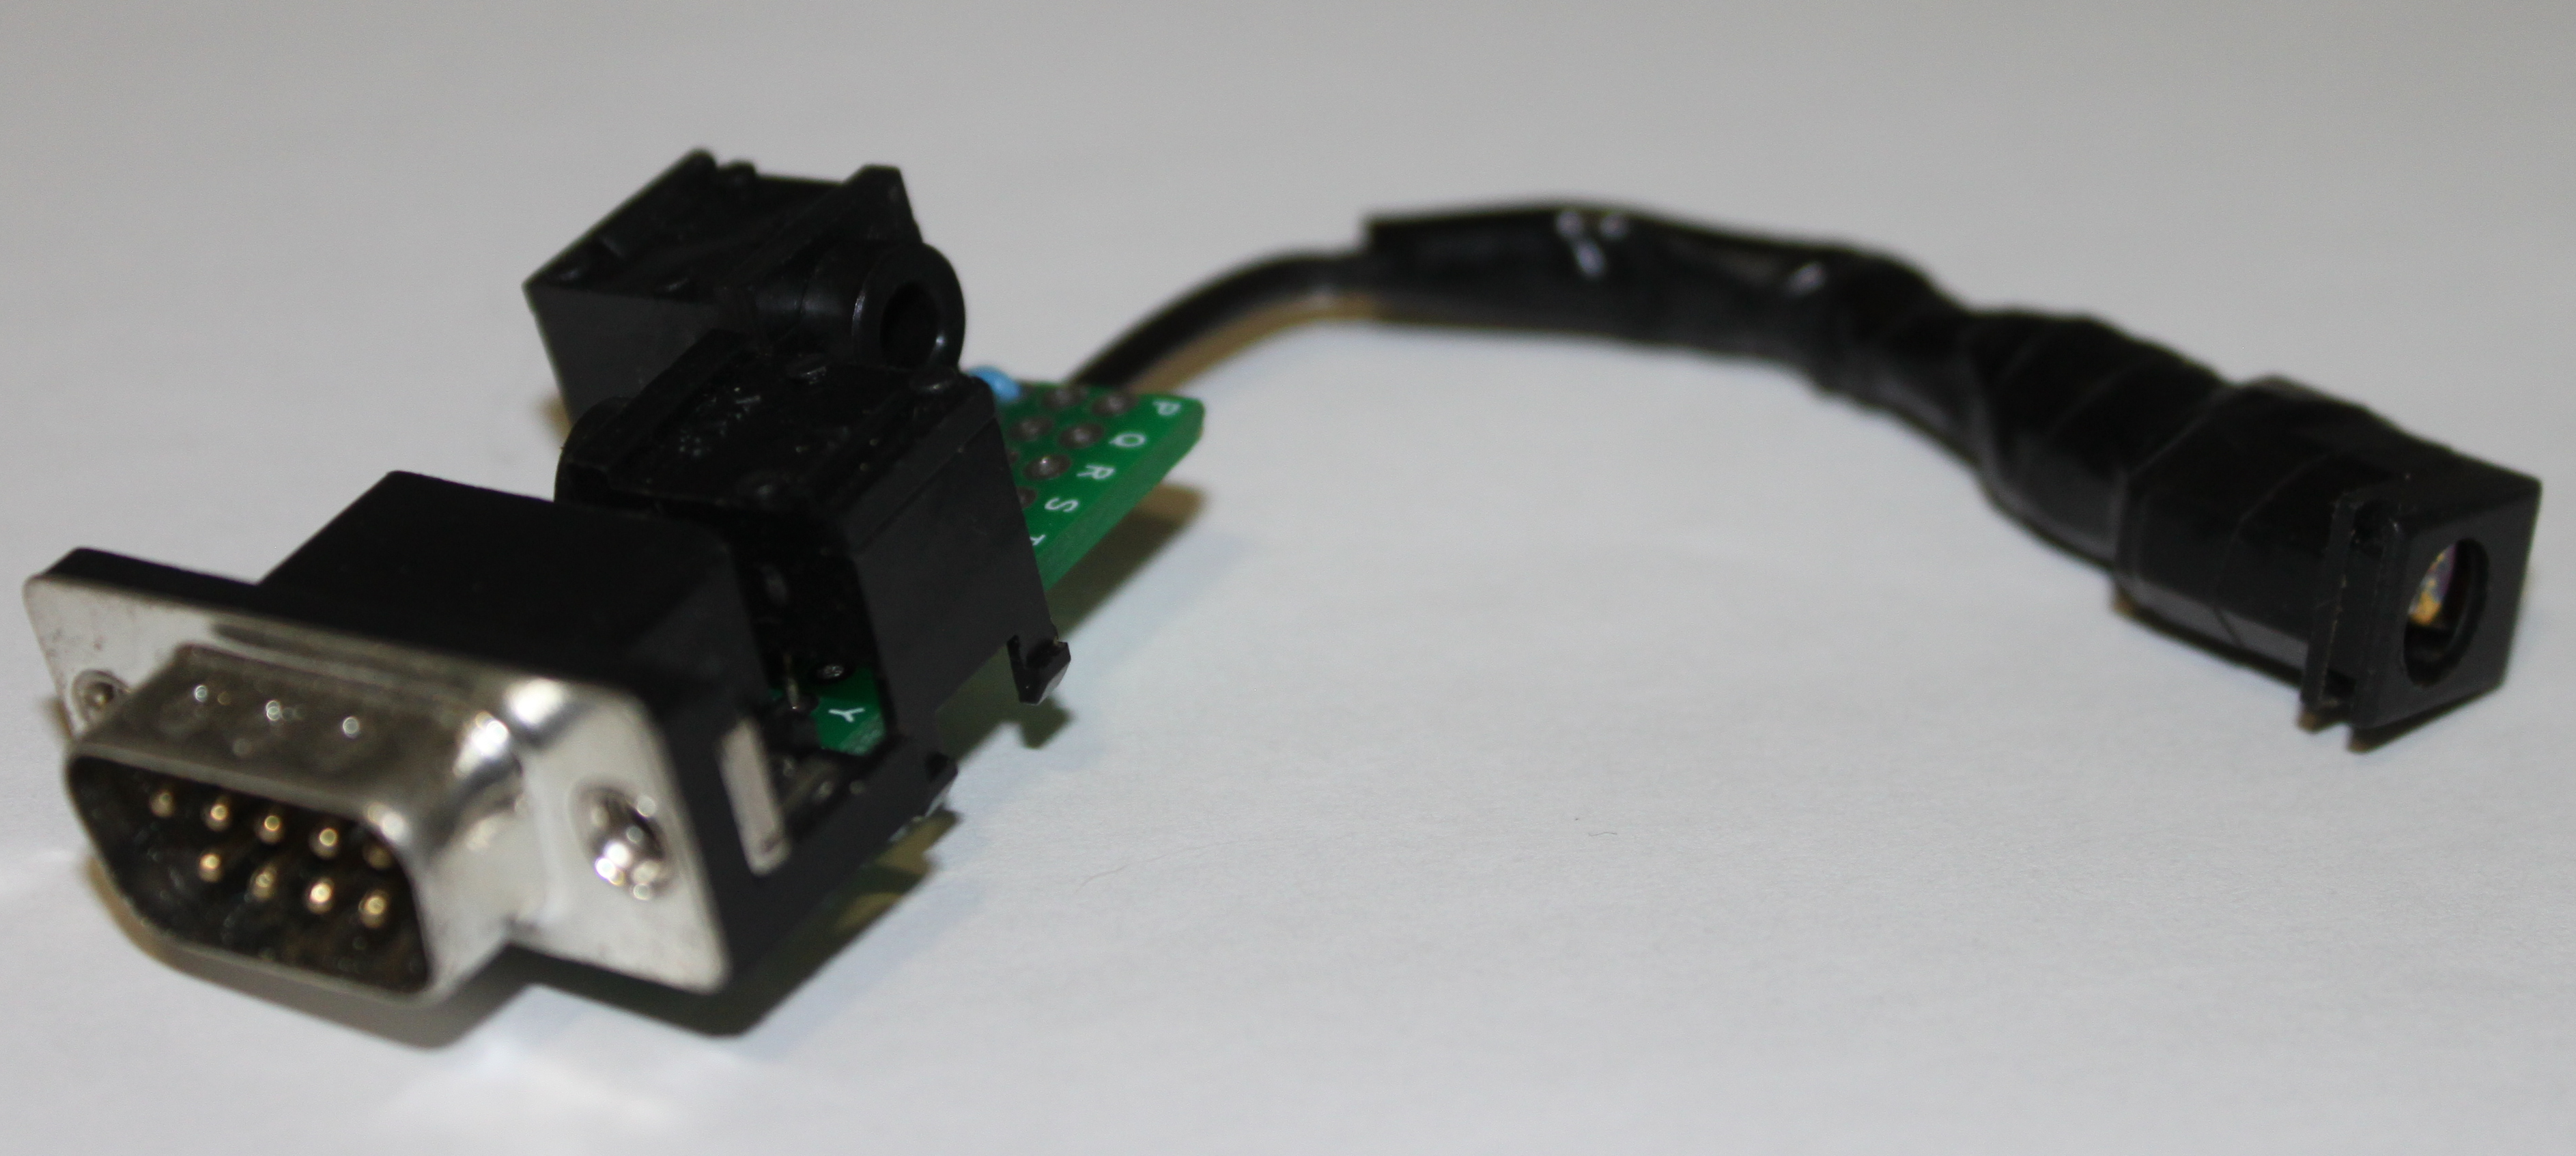
\includegraphics[width=0.75\linewidth]{images/BreakOutBoard.png} 
	\caption{Break-out board fabricated for hardware testing. There are two audio ports on the board; one for audio in and the other for audio out. On the right is the barrel jack for supplying power.}
   \label{BreakOutBoard}
\end{figure}

\subsection{Setting TNC Audio Levels}
During the testing, setting the audio level to be percisely correct for optimal performance would have been ideal. However, there is language in the user manuals for the various TNCs that is definitely up for interpretation. Such as in the MFJ-1278 manual which reads: "Continue to advance the volume control until there is approximately twice as much audio present at the receiver output $\langle$as the minimum$\rangle$" \cite{MFJ1278Man}. Additinally the manual for the Kantronics Kam Plus says: "Increase the volume control slightly from this point" \cite{KamPlusGettingStarted}. The volume level that was used for the audio provided to the TNCs was setting the laptop system volume to 50\% which worked out to about 1.1V peak-to-peak (Vpp). After doing some deeper reading of the individual TNC user manuals and verifying the expected results that were outlined, the approximate minimum optimal audio levels can be seen in Table \ref{TNCAudioLevels}.

\begin{table}
	\begin{center}
		\begin{tabular}{ | l | c | c | c | c | }
         \hline
			TNC & KamPlus & MFJ-1278 & PK-88 & PK-232 \\ \hline
			Level (Vpp) & 0.5 & 0.25 & 0.15 & 0.35 \\ \hline
		\end{tabular}
		\caption{Minimum Optimal TNC Input Audio Levels \cite{KamPlusGettingStarted,MFJ1278Man,PK88Man,Inc.2001}.}
		\label{TNCAudioLevels}
	\end{center}
\end{table}

\section{Software Testing Setup}
Included within the javAX25 suite was a testing application that could both generate and decode packets. However, it was limited to only being able to specify one audio file and one demodulation algorithm. Using this test file as a basis, a new testing application was created that allowed for the multiple demodulators to be compared side by side against multiple audio files with a single run of the application. In addition to the output being printed to the console, it was saved to a file. Having these features in the testing application allowed for a much more streamlined analysis of all the algorithms collectively and tuning individual algorithms. One very convenient aspect of programmatically testing is that it is very easy to add a loop to try a range of tuning parameters and then look at the results to decide what is the best option. All of the results listed in the following chapter are from the testing application and mechanism described here.

\chapter{Implementation}

This chapter will go through all of the implementation details of each demodulator implemented. They will be presented in order of complexity, with the more intricate ones presented last. This also will introduce them mostly chronologically since naive approaches allowed for more insight to be gained into the javAX25 software package before implementing more complicated algorithms. In addition to giving a brief overview of each implementation some performance data will be provided, but all of the data will be presented in the Results Chapter. As mentioned in the Demodulation Techniques Chapter, javAX25 was selected because of its availability and as such all of these implementation can be found in the author's Fork of the javAX25 GitHub repository in the following reference \cite{myJavAX25}. 

\section{Strict Zero Crossing Demodulator}
This approach used the technique of finding zero crossings and then using those to determine the period; from the period, the frequency was then calculated. For 1200Hz and 2200Hz tones zero crossings are expected every 833us and 455us respectively. If the resulting frequency after calculations was above 1700Hz it was assumed that a mark was present in the signal and if lower than 1700Hz a space must be present. Each zero crossing was found by determining if the signal was negative and changed to positive or if it was positive and changed to negative. Although this algorithm was only able to decode a little over half of the packets as some of the other algorithms, it proved to be an important stepping stone into javAX25 and allowed for preparation into restructuring the project for added modularity of the filtering. With the first implementation, Toledo's filters were not used and instead the previous three samples were averaged as a method of filtering to remove sample to sample noise.

\section{Floating Ground Zero Crossing Demodulator}
Building on the strict zero crossing algorithm the next zero crossing demodulator tried to use some more intelligence in finding the zero crossings through additional processing. One reason that the strict zero crossing approach was thought to have relatively poor results was due to the previously introduced challenge of DC offset. If the signal doesn't actually cross zero then it will be very hard to find the zero crossings. This new zero crossing method keeps a window of history (it was arbitrarily chosen to be one bit period) and from this collection of samples the average is taken to use this as the ground - or zero value. Instead of checking to see if the signal crosses zero, the signal is analyzed for going from either above to below or below to above this average value. This ended up having worse results than the strict zero crossing demodulator. This was due in part to the fact that 2200Hz signals - even when properly centered around zero - will not have an average of zero since it does not complete two fill periods within on bit period, which tainted the average.

\section{Windowed Zero Crossing Counting Demodulator}
With a good handle on utilizing zero crossing, a new approach was taken to keeping history. Instead of using the history to calculate where "zero" is, a new question was asked, "What if how many zero crossings within one period is observed?" If a window slightly shorter than one bit period is selected, then if there are only two crossings within the window that will correspond to a 1200Hz symbol being present. More crossings than two means that a 2200Hz symbol must be present. The thought behind taking this approach is that it would give some additional resiliency to noise by finding the average during that bit period through utilizing multiple zero crossing instead of individually analyzing every zero crossing. 

\section{Peak Detection Demodulator}
After making a simple zero crossing overly complicated, it was decided that maybe a different approach should be taken, specifically to look at a different part of the signal. It was considered that perhaps better performance could be achieved by looking at the peaks in the signal instead of the noisy zero crossing around ground, or not around ground if there are DC offset problems. Conveniently, the difference between two consecutive peaks will be equal to the period of the underlying signal. Although the methodology is the same as the zero crossing for converting the period to the actual frequency, it was perceived that this would give better results. It turns out that this method did not work as well as hoped due to the fact that local peaks were commonly discovered from the noise instead of the actual peak in the transmitted signal. More analysis into selecting a proper filter may give this approach better results.

\section{Derivative Zero Crossing Demodulator}
After a failure with the peak detection demodulator, a new approach was taken to finding "peaks." Instead of actually looking for the peaks, the zero crossing demodulator was revisited with a new spin. Instead of using the raw samples for determining the frequency using zero crossings, the derivative was to be used. The derivative was calculated by doing the same averaging as in the strict zero crossing approach and then subtracting the current average from the average two samples prior. It was thought that this would solve the DC offset problem for sure, but it turns out that this was not the larger problem. The problem was with using the zero crossing approach and this derivative implementation ended up having very similar results to the strict zero crossing with which one was better changing based off of pre-filtering.

\section{Goertzel Filter Demodulator}
Finally moving away from approaches utilizing zero crossing methodologies, an approach using a Goertzel filters was implemented. The implementation was very simple and corresponds with that outlined in the Demodulation Techniques Chapter. Since it has to be applied onto a set of data, a window size that was equal to one bit period was originally selected so as to make sure that the data being processed was only that of one frequency, but after analyzing the effect of the window size on performance, a window size of slightly longer than a bit period ended up being better. The optimal size was tested to be 135 percent of a bit period, and the reason why this worked better is because it gave more signal in the window for the filter to lock to. Essentially, the window was only extended 18 percent on each side of a bit period. This over-extension of the window is what led to being able to exceed the performance of the original correlator on unfiltered data.

\section{Phase Locked Loop Demodulator}
Next, the PLL demodulator was implemented. Using Lutus's python based software PLL initial testing was performed to see how it would work for tracking AX.25 signals \cite{Lutus2011}. Once the parameters were tuned sufficiently that it seemed to be staying locked onto the signal, it was ported over to java and actually run as a demodulator. Once inside of the javAX25 framework additional tuning was done programmatically instead of manually to further fine tune the performance. The final results were that it was not the winner, but comparable to the other top contenders, the Goertzel filter and correlation.

\section{Mixed Preclocking Demodulator}
Finally with numerous simple algorithms implemented it was time to try something much more complicated and also only possible in software. This approach and the name preclocking comes from an abbreviation for predetermined clocking where packets are analyzed a whole packet at a time. The start and end are found and then the clocking, and hence bit boundaries, are predetermined before the actual demodulation takes place on a baud by baud basis as opposed to a sample by sample basis. Each one of the preceding algorithms was on a sample by sample basis, meaning they had to make their best determination of bits elapsed using a little bit of history.

There are five steps to the demodulation in the Mixed Preclocking Demodulator. It was speculated that processing one packet at a time with the correct clocking to demodulate bit by bit would allow for very accurate demodulation.
\begin{enumerate}
\item Flags are found in the signal so that the demodulation can happen one packet at a time instead of just blindly trudging forward through the packet sample by sample.
\item The derivative of the whole packet is taken to  determine the zero crossings.
\item Frequency transitions are extrapolated from the derivative data.
\item The frequency transitions found in the packet are used to determine the clocking or bit boundaries.
\item The tone demodulation is done on a baud by baud basis.
\end{enumerate}

Although it was hoped that the results would be phenomenal, there were so many different methodologies being used that this preclocking demodulator was very difficult to tune. For instance the flags were found using the correlation approach, the transitions using a derivative, and the final demodulation using the zero crossings. What were thought to be the advantages ended up being the challenges, but as predicted it did well enough to still be considered one of the successful implementations. The intricate nature of this demodulator made it delicate, which was noticed during the testing through the fact that it would not decode any packets unless a bandpass filter was used on the incoming data.

\section{Goertzel Preclocking Demodulator}
After the first attempt at a preclocking approach, it was thought that perhaps using only one methodology to perform all the different steps of demodulation would be at the very least simpler, and ideally better. The perception that it might be better came from the fact that there was only one item to tune, the Goertzel Filter which had already shown good performance. Instead of having to worry about noise affecting zero crossings and the derivative potentially adding emphasis problems, only the filter had to be considered. Unfortunately, the number of packets that this method decoded was not as many as the first Goertzel approach or the previous preclocking. This was due to the fact that even though there was one underlying algorithm it was used in three separate instances, and each needed slightly different tuning. The three instances were for flag detection, frequency transition detection, and the the final bit by bit demodulation.

\section{Goertzel Exhaustive Preclocking Demodulator}
The final algorithm implemented was just a manner of verification, and another one that could be performed only in software. Instead of analyzing packets one at a time using flags as the start and end points, a whole array of data that had a length equal to the number of samples that a packet of the maximum length would have. Every time a few more samples came in, every single clocking was attempted on the large array of data just to see what packets could be decoded by exhaustively searching through the data. In terms of run time, this algorithm took much longer. For instance, the mixed preclocking and original Goertzel preclocking took 3 minutes and 5 seconds and 2:36 respectively to run, while this exhaustive search took 26:48 on the 25:49 Track 1 of the test suite. This means that a 2.1Ghz Intel i7 (i7-3612QM) could not process the audio file in less time than elapses during the content of the audio file. With that being the case, the result is that with live data this approach would not work since it would continuously fall behind. Gratefully, this approach only decoded an additional 15 packets that the Correlation, original Goertzel (non-preclocking), and PLL did not decode. This result could be used to make the argument that the few more packets decoded is not worth the vast number more CPU cycles it take to achieve it.


\chapter{Results}
This results chapter is meant as a mechanism to present all of the data that was collected on the performance of different demodulator. All of the demodulators that were tested in the course of this research will be shown whether that be dedicated hardware or software. The first results that will be shows are those of the dedicated hardware, being TNCs and Argent Data's Open Trackers. Following the hardware will be the software implementations. And following that will be some general comparisons between the hardware and software.

\section{Dedicated Hardware Results}
Before presenting all of the data on how many packets were correctly demodulated in each one of the five test files, each one of the pieces of hardware will listed.  In the scope of this research a total of 12 pieces of hardware were tested and they are Argent Data's Open Tracker 2, Open Tracker 3, Open Tracker USB, Open Tracker 3 Micro, Kantronics Kam, two Kantronics Kam Plus, two AEA PK-88, a PK-232, a PK-232MBX, and an MFJ-1278. Please note that on the figures Open Tracker will be abbreviated OT.

The first two tests consisting of clean packets - 40 generated from the Open Tracker and 200 using Toledo's suite - was relatively uninteresting. Essentially every piece of hardware decoded all 40 and all 200 packets. The only anomalies to this were that the Open Tracker USB was only able to decode 39 and 193 out of the 40 and 200 packet files respectively. Additionally the Open Tracker 3 Micro missed one packet in the 200 packet file to only decode 199. For these since there is no real way to debug and see the cause of decoding relatively fewer or more packets just the data is presented as it was measured to allow for comparison to the software. This will continue to be the case for the remainder of this hardware section.

Following the two easy files the next file is same content as the file with 40 packets in it with the only difference being that noise was progressively added. In Figure \ref{allHardwareOT3Noise} the two PK-88s stand out for being able to decode 25 of the 40 packets in this file.

 \begin{figure}
  \centering
	\includegraphics[width=0.75\linewidth]{images/PerformanceofAllHardwareonOT3TestwithNoise.png} 
	\caption{Number of packets successfully decoded for all tested hardware on Open Tracker 3 test file with noise.}
   \label{allHardwareOT3Noise}
\end{figure}

The next two files are the ones that were used most extensively in the testing for comparison and tuning. Primarily the first which is just a recording of traffic off the air. They are Track 1 and 2 from the APRS CD mentioned in the Demodulator Benchmarking Chapter. The results from Track 1 are in Figure \ref{allHardwareTrack1} and Track 2 in Figure \ref{allHardwareTrack2}. The top three of the hardware on Track 1 was the PK-88 (2) with 1007 packets decoded, the Kam with 988 Packets, and the Kam Plus (2) with 985 Packets. For Track 2 the top hardware was the Kam Plus (2) with 998, the Kam Plus (1) with 967, and the Kam with 938.

 \begin{figure}
  \centering
	\includegraphics[width=0.75\linewidth]{images/PerformanceofAllHardwareonTrack1.png} 
	\caption{Number of packets successfully decoded for all tested hardware on Open Tracker 3 test file with noise.}
   \label{allHardwareTrack1}
\end{figure}

 \begin{figure}
  \centering
	\includegraphics[width=0.75\linewidth]{images/PerformanceofAllHardwareonTrack2.png} 
	\caption{Number of packets successfully decoded for all tested hardware on Open Tracker 3 test file with noise.}
   \label{allHardwareTrack2}
\end{figure}

Using these results the best numbers for the hardware were 40 packets decoded from the Open Track 3 test, 200 from the javAX25 generated file, 25 from the Open Tracer 2 test with added noise, 1007 from Track 1 of the LA test suite, and 998 from Track 2.

\section{Software Results}

\subsection{Hardware and Software Comparisons}


\chapter{Future Work}


%%%%%%%%%%%%%%%%%%%%%%%%%%%%%%%%%%%%%%%%%
%All of this should be redone...
%%%%%%%%%%%%%%%%%%%%%%%%%%%%%%%%%%%%%%%%%
For the future work for the software based demodulation algorithms, more parameter adjustment can be made to try and better fine tune the performance. For instance there are a handful of parameters in the windowed zero crossing algorithm that can be modified. As can be imagined with the Preclocking algorithm and its six stages there are even more parameters that are available for tweaking. Even with the brief time spent modifying the parameters more successfully decoded packets were acquired. Furthermore with the Preclocking algorithm, instead of only using the zero crossing frequencies inside the determined baud period a correlation of the likelihood of the two frequencies could be used as well like in Toledo�s demodulation technique. Also, continuing to investigate the source of corrupted packets and identifying corrections to improve the algorithm can be made. The current results with the Preclocking came from investigating only a handful of packets. The process is tedious and time consuming, but contains the potential for further improvements.

In addition to tweaking parameters, filtering, thresholds, etc. on the implemented algorithms there is also work that can be done on the testing, the framework, and on implementation of different algorithms.


\section{Potential Modifications to the Testing Methods}

The testing class that is currently in place was enough to meet the testing needs and see how many packets were successfully decoded by the software based algorithms. However, there is a lot more work that can be put into the testing. For instance it would be beneficial to be able just run a complete test with all of the desired input files instead of having to rerun the software for each individual file and have the testing class just print out all of the statistics at the end.

Additionally, although a little work was put into this already, it would be nice to know exactly which packets are decoded by some algorithms and not by others so that the signal can be looked at in those specific portions in order to determine what the causes of the weaknesses of the algorithm might be. It is very difficult to know what is the maximum number of packets that can be decoded from the real life test data, but as the software algorithm numbers are still under the TNCs, there are improvements to be made.

Once the packet outputs can be compared side by side it will be clearer what are the strengths and weaknesses of each algorithm. Additionally, once the packets that the software based algorithms could not demodulate are identified it would be nice to be able to look at differences between the bit stream of the correct packet and the improperly demodulated packet.

Finally, similar to how Toledo has varying parameters for his filters it would be interesting to have the program just go through and self-optimize itself. Have the tweakable parameters run through a range of values and then do analysis on the values of the internal parameters that resulted in the most decoded packets.

\section{Potential Modifications to the JavaAX25 Framework}

In addition to modifying the testing framework there is also some work that can be done on cleaning up the whole JavaAX25 package as a whole. Currently there is enough there in order to make the system work, but there are improvements that can be made in order to separate distinct algorithm logic better as well as different functional groups. For instance there is a lot of code that exists in all of the classes due to the fact that once the transitions are found calculating the number of bits and constructing the packet is always the same. If this code was put in the abstract class that all the demodulators extend from it would make the code base as a whole more robust and easier to navigate for new users to do their own analysis.

\section{Other Algorithms for Consideration}

Once the testing and framework are built into a more robust state then the focus, which is in improving the demodulation algorithms can be focused on more exclusively. From the research it can be concluded that the correlation based demodulation is as the paper title indicates a fairly �High Performance Sound Card AX.25 Modem.� However the Preclocking algorithm showed good results when using the derivative which potentially eliminates the need to run two algorithms side by side, one with an emphasis filter and one without. Using the same correlation logic on the filtered derivative instead of on the original signal is then one option to consider as a future algorithm.

Another advantage of the Preclocking algorithm was the fact that the software only has to make decisions on a single baud as opposed to all of the samples it has received thus far. If instead of using the frequencies that were extracted from the derivative data to determine the clocking, the correlation was used this may also show improvements. Basically it could be the best of both worlds since the Preclocking and correlation have already proved to work well together. 

There are many other permutations and combinations of the different algorithms that can be considered in order to try and make the algorithm as good as possible and these are only two small ideas. From the research in this paper hopefully the next implemented algorithm will take the high points and use them all together to continue to improve the software based demodulator. 

\chapter{Conclusion}

%%%Presumably the conclusion will be different after the results have been formed...
This research has proved and presented several demodulation techniques that do not seem to have been considered when doing software based demodulation previously on APRS. Most importantly, the premise that software based demodulators are not as good as the hardware ones holds meaning that there is still the potential for work to be done on the software based demodulators in order to increase the number of successfully decoded packets to compete even closer with hardware. The project also further demonstrates that decoding in software is not a limitation, but can be further refined.

\bibliographystyle{plain}
\bibliography{../references}

\end{document}
